% REMEMBER: You must not plagiarise anything in your report. Be extremely careful.

\documentclass{l4proj}

    
%
% put any additional packages here
%

\begin{document}

%==============================================================================
%% METADATA
\title{Level 4 Project Report Template}
\author{John H. Williamson}
\date{September 14, 2018}

\maketitle

%==============================================================================
%% ABSTRACT
\begin{abstract}
    Every abstract follows a similar pattern. Motivate; set aims; describe work; explain results.
    \vskip 0.5em
    ``XYZ is bad. This project investigated ABC to determine if it was better. 
    ABC used XXX and YYY to implement ZZZ. This is particularly interesting as XXX and YYY have
    never been used together. It was found that  
    ABC was 20\% better than XYZ, though it caused rabies in half of subjects.''
    \begin{itemize}
        \item what is LBD?
        \item what will this project do?
        \item what is the result of this project?
    \end{itemize}
\end{abstract}

%==============================================================================

% EDUCATION REUSE CONSENT FORM
% If you consent to your project being shown to future students for educational purposes
% then insert your name and the date below to  sign the education use form that appears in the front of the document. 
% You must explicitly give consent if you wish to do so.
% If you sign, your project may be included in the Hall of Fame if it scores particularly highly.
%
% Please note that you are under no obligation to sign 
% this declaration, but doing so would help future students.
%
\def\consentname {Timothy Baldock} % your full name
\def\consentdate {30 January 2024} % the date you agree
%
\educationalconsent


%==============================================================================
\tableofcontents

%==============================================================================
%% Notes on formatting
%==============================================================================
% The first page, abstract and table of contents are numbered using Roman numerals and are not
% included in the page count. 
%
% From now on pages are numbered
% using Arabic numerals. Therefore, immediately after the first call to \chapter we need the call
% \pagenumbering{arabic} and this should be called once only in the document. 
%
% Do not alter the bibliography style.
%
% The first Chapter should then be on page 1. You are allowed 40 pages for a 40 credit project and 30 pages for a 
% 20 credit report. This includes everything numbered in Arabic numerals (excluding front matter) up
% to but excluding the appendices and bibliography.
%
% You must not alter text size (it is currently 10pt) or alter margins or spacing.
%
%
%==================================================================================================================================
%
% IMPORTANT
% The chapter headings here are **suggestions**. You don't have to follow this model if
% it doesn't fit your project. Every project should have an introduction and conclusion,
% however. 
%
%==================================================================================================================================
\chapter{Introduction}

% reset page numbering. Don't remove this!
\pagenumbering{arabic} 

\section{Motivation}
\begin{itemize}
    \item Scale of research
    \item Cost of machine learning
\end{itemize}

\section{Aims}
\begin{itemize}
    \item Explore different aspects of MeSH tags in lbd
    \item Give pointers on what variations are useful
\end{itemize}

\section{Dissertation Outline}
\begin{itemize}
    \item Background
    \item Analysis
    \item Implementation
    \item Evaluation
    \item Conclusion
\end{itemize}

%==================================================================================================================================
\chapter{Background}

\section{Increase in Research Rate}

The global research rate is increasing. This is in part fueled by the global spending on research and development has increased to 2.4 trillion dollars in 2020 from only 675 billion in 2000 as reported by the Congressional Research Service (2022). As research across the world continues to grow, so to does our accumulated knowledge grow. According to Bornmann and Lutz (2015) \textbf{ref}, the rate of research increased exponentially between 1980 and 2013, with a growth rate of about 3\% for global scientific publications in this time frame. With an ever growing repository of information it becomes more difficult to accumulate expertise in a field. This is further exacerbated by the increasing rate of research which also makes it trickier for individual experts to stay up to date with developments in their field. \\ 

The result of this, is a narrowing of expertise as discussed by Swanson et al. \textbf{ref}. To become expert in a field requires increasingly more time to be spent on a narrower area of a field. A consequence of this is that individuals can benefit less from their wider understanding of their field as not only can they spend less time learning about the broader subject but also the required time taken to properly develop knowledge in other parts of their field increases.\\ 

\section{Introduction of Literature Based Discovery}

Here is where literature based discovery, LBD, comes in. LBD is the idea that we can use this vast and ever growing database to generate hypothesis for future work. Henry and McInnes \textbf{ref} provide many examples of LBD's applications and achievements including identifying potential treatments for cancer and finding treatments for cataracts. Biomedical research is the field in which LBD is most utilised, but there are numerous instances of its use in other fields. Aamot's work with using it for oceanographic climate science is a case of LBD being applied to another field with its application in studying climate change. Given the increasing quantity and funding of research, being able to effectively generate hypothesis by linking different areas expertise will only become more crucial.\\  

\section{PubMed}

PubMed is a system to help with the organising and searching of life science and biomedical literature. It was created by the National Center for Biotechnology Information and contains the abstract and other key information of over 36 million publications. The primary feature of PubMed is MEDLINE, a system containing citations from selected journals and articles indexed by MeSH tags. \\

\subsection{MeSH Tags}

MeSH tags are a system of labels used to identify and categorise biomedical articles in the PubMed database. MeSH tags provide a standardized set of terms to describe the subject matter of articles. This ensures consistency in indexing and searching across different databases and publications and is controlled by the National Library of Medicine. They were made publically available in 1996 and have been key to searching and organising biomedical literature since. By keeping the scope of terms controlled, the National Library of Medicine can ensure that similar concepts are labelled in a consistent manner, irrespective of different cultures and languages across the world. This is very important in a globally researched subject to establish a standard format to research categorization. The MeSH database is regularly updated and expanded to reflect advances in biomedical research and changes in terminology. New terms are added, and existing terms are revised to ensure accuracy and relevance in a continuously evolving field. \\

\begin{figure}[h]
    \centering
    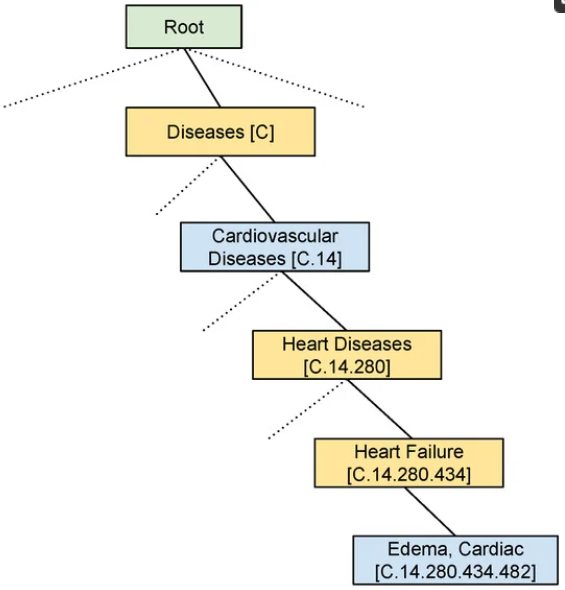
\includegraphics[width=0.6\linewidth]{images/mesh_label.png}
    \caption{image from: Integrating PubMed Label Hierarchy Knowledge into a Complex Hierarchical Deep Neural Network}
    \label{fig:mesh}
\end{figure}

 The MeSH tag system is organised in a hierarchical tree structure. One advantage of this is it allows users to navigate through broader categories down to more specific terms. For example, the term "Diseases" is a broad category, under which you may find more specific terms like "Cardiovascular Diseases" and so on. With this, users can search for whatever level of specificity they require when exploring literature. Not only will this allow expert users to effectively filter down to exactly what they need, but also, less experienced users can use terms they are more familiar with to access larger sections of research. This process can even be conducted progressively, with users walking through the tree of terms to identify the best term for them to use. \\

 By using this tree structure, MeSH also helps facilitate an easier and more consistent labelling of literature. It is easier to label data as a user does not need to select "Diseases" as well as "Cardiovascular Diseases". Instead, by selecting the most specific term that is relevant, they imply all the higher order terms that path directly to that term. For example, in  \Cref{fig:mesh}, selecting "Heart Failure" would implicitly label the paper with "Diseases", Cardiovascular Diseases" and "Heart Diseases". However, it would not label it with "Edema, Cardiac". This also keeps labelling of papers consistent, as researchers only need to select the most specific term for their paper, to then automatically assign a set of other relevant terms. Ensuring that all papers about "Heart Diseases" are also labelled with "Diseases" is not only important for consistent search results, but also for categorizing research for the purposes of using it as data. \\

 A significant issue in natural language processing (NLP) of expert fields is getting data labeled by experts. This can be a very time intensive, yet boring task and so it is difficult and expensive to get experts in a particular field to label data for classification. This problem is exacerbated by modern NLP systems using vast quantities of data from a huge array of fields, many of which might well require expert understanding. To find, convince and pay experts from this many different fields is an impossible task and so finding data that does not require labelling is crucial to effectively developing such systems. \\
 
 MeSH tags work very well as data labels. Since they are a controlled vocabulary, they ensure that papers that overlap in an area will be labelled consistently with each other. Furthermore, they are explicitly labelled by experts and so have a great value as accurate and useful data. For a field like biomedical science, that is so complicated and can get very niche, this is an incredibly crucial factor for LBD research and development. Having in a place such a well developed data labelling system is probably a significant factor in why LBD has seen particular development in the field of biomedical and life sciences. \\

 Efficiency is a significant concern in data analysis. Often vast quantities of data is being processed and stored, so making sure to reduce this burden on the system is important. Not only will reducing data in a meaningful manner help with reducing run time and storage space, it also can help improve quality of results, as the noise in the data is reduced. Noise is the idea of data points that bulk out data sets without adding much meaningful information that can be used to improve results. Here are some examples of noise in data.
\\ 
\begin{itemize}
    \item \textbf{Sensor Noise}, In data collected from sensors such as cameras or microphones, noise can be caused by electrical interference, fluctuations in the environment, or inaccuracies in the sensor itself. 
    \item \textbf{Stop words}, In NLP, many words are so common they are redundant. These are categorised as stop words and it is common practice to filter the most common ones from data. This can range from removing a few hundred to a few thousand words, depending on the context of the task.
    \item \textbf{Transmission Noise}Data transmitted over networks or communication channels can be corrupted by interference, distortion, or packet loss. \\
\end{itemize}

MeSH tags are very efficient as data. They can be used to filter massive documents of text down into a handful of key terms that best describe the document. This will therefore save researchers using them a significant amount of time that is normally spent filtering data down into something meaningful, and since these terms are carefully selected by experts, reduce the risk that the filtering might remove vital information from the data. Furthermore, MeSH tags can be filtered down further, either by filtering for tags from certain branches of the tag tree, or by only using major topic tags, that are used to represent the main focus of a paper. \\

Despite these benefits, MeSH tags do have drawbacks when used as data in this way. Since they are primarily tags for searching and categorising research papers, they are selected with this in mind. Information that is not deemed relevant for someone searching for this paper will therefore not be included in the MeSH tags. They are not selected to cover all areas of a paper for the purpose of LBD and so might not include information that actually could have helped identify links between research. Because of this there is extensive research in the field of LBD in Biomedical science that uses more than just MeSH tags, for example the work done by Lever et al. where they use the titles and abstracts of papers to find coocurrences. 

\section{Swanson's ABC System}

\begin{figure}
    \centering
    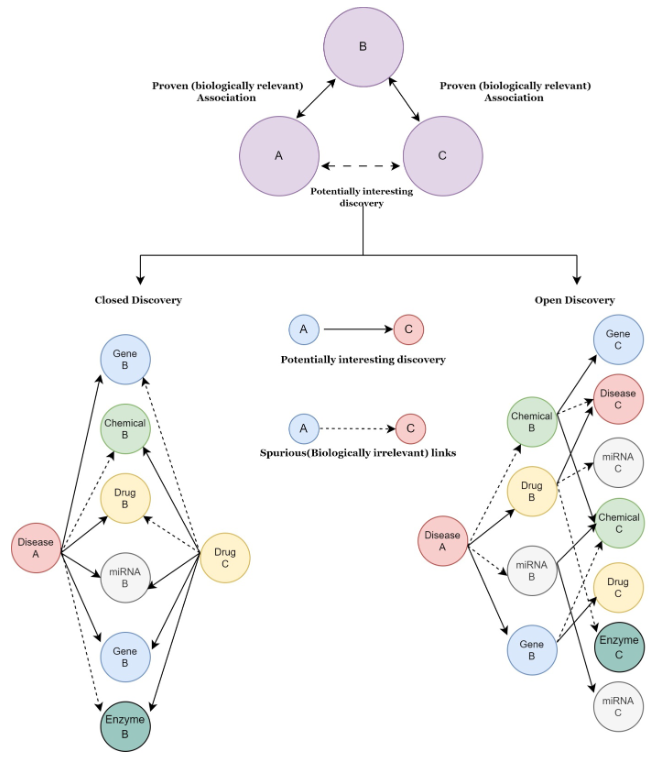
\includegraphics[width=\linewidth]{images/abc_open_closed.png}
    \caption{image from: Literature Based Discovery (LBD): Towards Hypothesis Generation and Knowledge Discovery in Biomedical Text Mining}
    \label{fig:open_closed}
\end{figure}

LBD is founded on Swanson's ABC approach. In this approach, if concepts A and B have an established relationship, and concepts B and C do too, then there may well be a transitive relationship between A and C. This is visualised at the top of \Cref{fig:open_closed} where A and B, and B and C are linked by proven association and so the link between A and C might be a potentially interesting discovery. In particular, this system is interested in circumstances where no relationship between A and C has been previously established as this might therefore be a new connection that could be discovered. An example of this being successfully implemented by Swanson himself would be his discovery of using fish oil to treat Raynard's disease. \\

\subsection{Open Discovery}

Open and closed discovery are the two main methods of Swanson's ABC system. Open discovery involves the user to have an identified concept A for which to discover possible C concepts. This can be done by identifying all the possible C concepts that are not linked to the original A but have at least one B concept in common with A. The connection between A and each C can then be evaluated by some metric and used to sort the possible C concepts in some way so that they can be returned to the user in meaningful manner. In this way, Open discovery can be used to answer the questions of what concepts are connected indirectly to a given concept and how they might compare to each other. \\

\subsection{Closed Discovery}

Closed discovery, on the other hand, seeks to answer entirely different questions. This system requires pre-given A and C concepts so that the B connections between them can be discovered. This allows the user to check if any common ground can be found between two concepts that they might suspect have a connection. This could even be generalised beyond unconnected concepts, it could be used to explore new ways two concepts, that have pre-existing connections, might be overlapping. Closed discovery therefore asks the question of how or why two concepts are connected. The two concepts do not have to exist in isolation of each other. In fact, since they answer very different questions they can be used in combination with each other to first discover new connections and then to explore why those concepts are connected. In this way Swanson created an effective and comprehensive approach to LBD, laying the groundwork for the development that followed. \\ 

\section{Discovery Methods}

\begin{figure}[h]
    \centering
    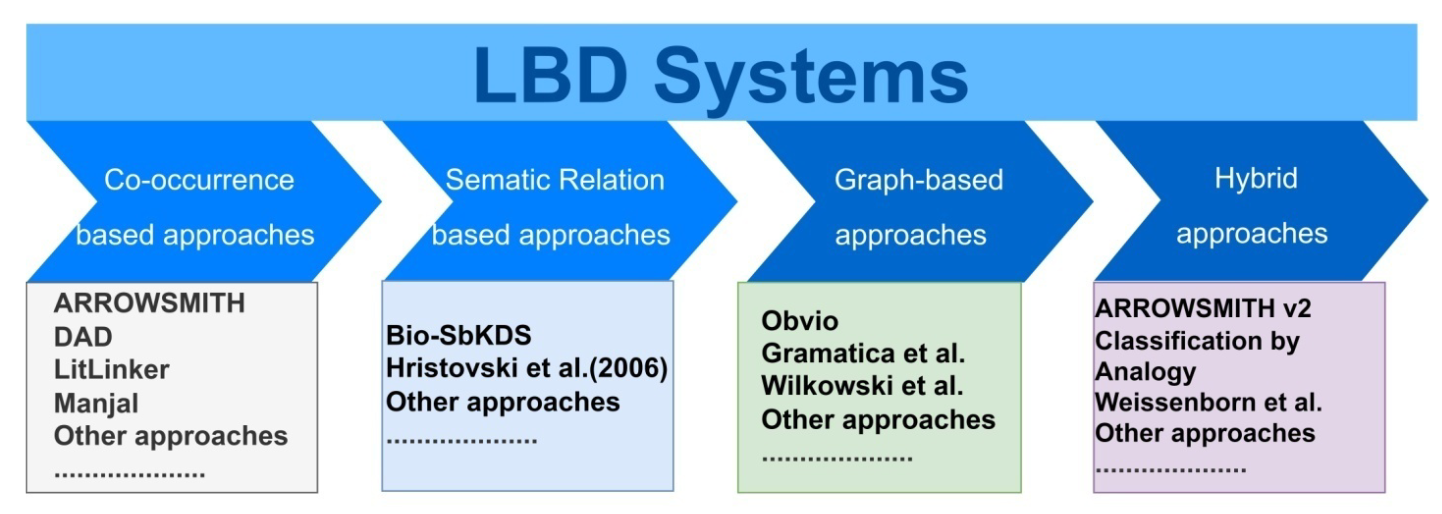
\includegraphics[width=\linewidth]{images/lbd_discovery_methods.png}
    \caption{image from: Literature Based Discovery (LBD): Towards Hypothesis Generation and Knowledge Discovery in Biomedical Text Mining}
    \label{fig:discovery_methods}
\end{figure}

Ultimately LBD depends on the proficiency of its discovery methods. Furthermore, for LBD to grow in use and to keep up with developing data analysis techniques, it must continue to improve the systems of discovery. \Cref{fig:discovery_methods} displays a rough outline of the progression of LBD systems and provides some umbrella concepts that allow the grouping of similar designs. There are have been several different approaches over the years which are worth exploring further. \\

\subsection{Co-occurence Approaches}

Using this ABC system, Swanson went on to developed the Arrowsmith search system. This is a co-occurence based system, where links between concepts are determined by if they both occure in the same paper's title. The objective of this tool is to make the ABC system more accessible and usable for researchers to actually use without having to build their own version of the system from scratch. The system implements the closed discovery system, allowing researchers to explore links between two pre-chosen concepts that they are looking to explore. \\

It functions by searching article titles in Medline, a biomedical database of citations and abstracts. It searches these titles for terms A and C, and returns a file for each respective term containing all of the titles with that term. The next step is for the Arrowsmith software to compare the two files and create a list of all 'B' terms that appear on both files. From here a stop word list of the 5000 most common terms is used to filter out the obviously redundant words from the list. \\

At this stage, the user can then filter the list further by taking out terms that they know are not relevant or interesting. Furthermore, the list can be automatically filtered further to only give terms that appear at least twice in both of the A and C files. This gives the user an easier way to significantly reduce the returned terms if they are dealing with a particularly long list. Using this finalised list, the system will return a list of titles containing both the A and B terms, and the B and C terms. From this, the user will be able to determine if they think there are any links between these concepts worth exploring. \\

In this way, Arrowsmith can be a useful tool for exploring connections between concepts. This is irrespective of whether or not there is a pre-existing connection between concepts A and C. It could for example be used to discover new links between two concepts that we already know are connected but want to explore further. However, a draw back of this system is that it is heavily reliant on the user being an expert in the field and having a wealth of experience at reading and understanding biomedical publications. \\ 

\subsection{Semantic Relation Approaches}

Another approach to LBD is utilising semantic relations to create more confident and accurate predictions. Hu et al. developed a system called Bio-sbKDS, Biomedical Semantic-based Knowledge Discovery System, that uses biomedical ontologies to try to fully automate the process of refining predictions. The benefit of this is it should greatly reduce the time and effort an expert would have to input to produce a meaningful result. By using semantic networks such as UMLS, Unified Medical Language System, the system can better identify connections that are worth investigating. In this way, this system implements Swanson's open discovery system, allowing users to discover concepts linked by specific relationships. To make these predictions, Bio-sbKDS takes in the following information from the user. 
\\
\begin{itemize}
    \item \textbf{Starting concept}, a keyword to represent the concept that the user wants to discover concepts that link to it. 
    \item \textbf{Semantic relationship}, the desired relationship that the user is interested in between the given concept and the discovered concepts. 
    \item \textbf{Date range}, a set of dates to limit the searched publications to. \\
\end{itemize}

Using these inputs, the user is able to significantly focus the output of the system towards what they are looking for. Furthermore, by reducing the date range to a relevant window for their particular research, the user can significantly cut down on the time taken for the system to process the data. \\

\subsection{Graph-based Approaches}

One aspect of graph based approaches is the idea of formatting and storing the information as a graph. This would be instead of the standard relational tables used for SQL, structured query language, as these tables don't make as much sense for data that is in the form of a network as opposed to distinct objects. Instead, if this can data can be formatted in storage as a graph, it could be more straightforward and more effective for accessing in LBD. \\

With this in mind, Hristovski et al. used Neo4j to graph database for LBD. Neo4j is a noSQL, commonly thought of as not only SQL, technology that allows the creation of a database that stores data in the form of a graph comprised of nodes and edges. Neo4j therefore has its own query language, Cypher, for accessing its data. With this query language, both open and closed discovery can be implemented on the database, allowing the previously described systems to be re-implemented using this technology. Cypher has the functionality to satisfy these systems, as it can both run simple commands that only care about co-occurrence, or more complicated ones that filter by concept and semantic relationship type. \\

However, implementation of this system did face some problems. When using the LOAD CSV command, for loading text data into the system, it failed to load all of the data, only managing the first few million instances. In addition, if the user wishes to place further stipulations on the nature of the concepts and relationships they want returned, the authors found that the queries would take longer to process. When the researchers built this system in 2015, Neo4j was version 2.1.6 and had two types of indexing, legacy indexes and schema indexes. The legacy indexes are not recommended as they are difficult to use, but they provide the desired text, node, and relational indexing. The ability to fully index text and relations is not provided by the recommended schema index. \\

\section{Machine Learning}


In the realm of data science, machine learning has emerged in a prominent role. Particularly it is used in extracting insights and predictions from especially vast and complex datasets. This is due to the inability of traditional algorithms ability to effectively run on such data, so creating the requirement for a different system. Its applications span various domains, including:
\\
\begin{itemize}
    \item \textbf{Recommender Systems}, where algorithms forecast future trends or behaviors based on historical data.
    \item \textbf{Classification and Clustering}, used for grouping similar data points or categorizing new instances into predefined classes. 
    \item \textbf{Natural Language Processing}, enabling computers to understand, interpret, and generate human language. 
    \item \textbf{Computer Vision}, developing machines ability to analyze and interpret visual data such as images and videos. \\
\end{itemize}
The continued success of machine learning across a variety of fields has continued to accelerate its development and applications. \\

\subsection{Environmental costs}

In 2022, Wu et al. conducted a holistic evaluation of the environmental costs and impacts of machine learning. Their key takeaway on the growth of AI is as follows: \\

\begin{quote}
    The Growth of AI: Deep learning has witnessed an exponential growth in training data, model parameters, and system resources over the recent years. The amount of data for AI has grown by 2.4×, leading to 3.2× increase in the data ingestion bandwidth demand. Recommendation model sizes have increased by 20× between 2019 and 2021. The explosive growth in AI use cases has driven 2.9× and 2.5× capacity increases for AI training and inference at Meta over the recent 18 months, respectively. \\
\end{quote}

This represents an incredible increase in scale, particularly for recommendation models used in often for LBD. An increase by a factor of 20 in model sizes over just two years is a massive difference in quantity that needs addressing. Fortunately, in the same paper, Wu et al. go on to discuss solutions to this problem. They propose that a key step to tackilng carbon emmissions is optimization of these systems. \\

\begin{quote}
    Optimization across the axes of algorithms, platforms, infrastructures, hardware can significantly reduce the operational carbon footprint for the universal translation model by 810×. Along with other efficiency optimization at-scale, this has translated into 25.8\% operational energy footprint reduction over the two-year period.\\
\end{quote}

This is part of the holistic solution they propose to reducing the footprint of AI which entails looking at these systems from data collection all the way through to training. Furthermore, the cost of manufacturing the hardware required for these systems is key given drive for producing ever better specialist hardware inspired by a boom in AI popularity.\\

\subsection{Matrix Factorization}

Matrix factorization is a technique in machine learning and linear algebra often used for recommendation systems. At its core, matrix factorization involves decomposing a matrix into a product of two or more matrices, with the goal of revealing hidden patterns or structures within the data. \\

\begin{figure}[h]
    \centering
    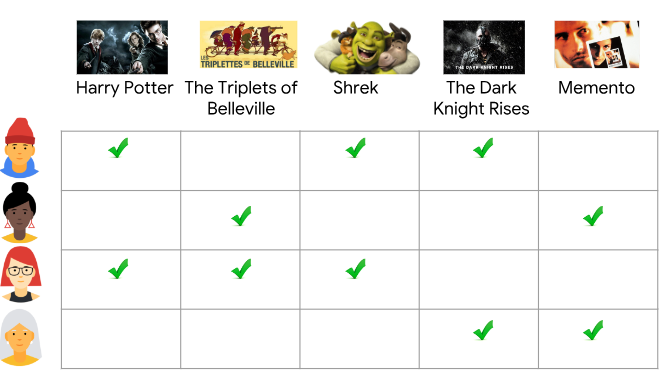
\includegraphics[width=\linewidth]{images/matrix_fact_example.png}
    \caption{image from: https://developers.google.com/machine-learning/recommendation/collaborative/matrix}
    \label{fig:matrix_fact_example}
\end{figure}

A common application of matrix factorization is collaborative filtering in recommendation systems. Here the matrix represents users' ratings for items (e.g., movies or products) as seen in \Cref{fig:matrix_fact_example}. This is an example of binary data in matrix, a user either likes or does not like a movie. However this system can also be used for more complicated relationships such as a rating. There is the limiting factor of the relationship must be represented as a singular numeric value, you could not have a matrix of text reviews, or set of numbers without first reducing them down to a single value. By decomposing this matrix into two lower-dimensional matrices, representing users and items, the algorithm can identify latent features that capture users' preferences and item characteristics. This allows for predicting missing ratings and generating personalized recommendations for users. \\

Koren et al. describe a model of matrix factorization for recommender systems.

\subsection{Graph Neural Networks}

Graphs used in LBD have already been introduced, but to generalise momentarily, graphs generally compose of three key forms of information:
\\
\begin{itemize}
    \item \textbf{Vertex (V)}, attributes that form the nodes of the and tend to represent objects such as people or movies.
    \item \textbf{Edge (V)}, attributes that link the graph together and tend to represent relationships between the nodes such as distance or likes. 
    \item \textbf{Global (U)}, attributes that summarize the overall state of the graph, such as number of nodes, number of edges or density. \\
\end{itemize}

With these simple attributes, a huge array of different data forms can be represented in graphs. Some things fit this really naturally such as a map, with locations and nodes and edges as distances, some things are more abstract, such as text, with words as nodes and the flow and structure represented by edges. \\

The objective of a graph neural network (GNN), is to try to learn hidden or general information implied by the graph that is not obvious to see. For example, given a set of movies that a user likes, predicting what would be other movies they would want to watch. Traditionally this would be done by categorising movies into genres, so that if a user watches a lot of action movies, then the system would recommend other action movies. However, GNNs can pick up on more subtle information, maybe users who like movies A, B and C also tend to like movie D from an entirely different genre. This allows systems to propose much more focused, accurate, and personal recommendations to users than previously. \\

\begin{figure}[h]
    \centering
    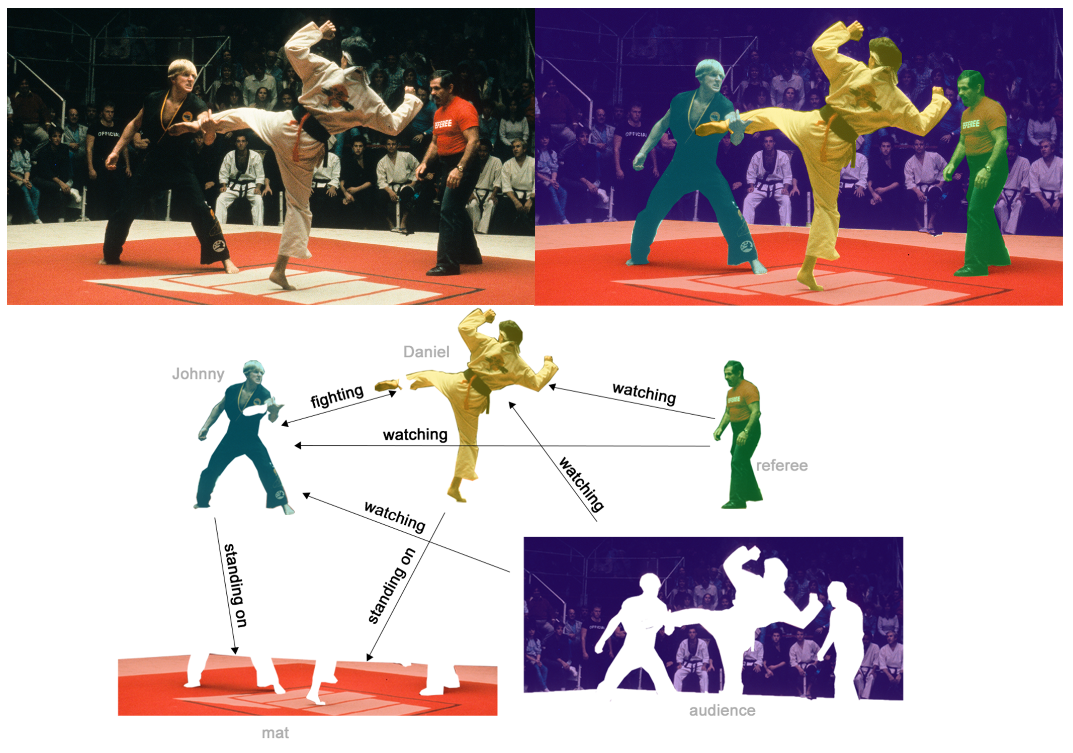
\includegraphics[width=\linewidth]{images/image_recognition.png}
    \caption{image from: https://distill.pub/2021/gnn-intro/}
    \label{fig:image_recogniton}
\end{figure}

In recommender systems, the objective is in completing edge-level tasks. That is to say, trying to establish, understand, and ultimately predict relationships between different nodes. An example of this can be seen in \Cref{fig:image_recogniton}, where the image is represented as a graph in order to understand it and even to understand the relationship between components with the image. This will allow complicated and data expensive things like images to be reduced down to very simple and small objects like a graph that can be much more easily processed.
%==================================================================================================================================
\chapter{Analysis}
\section{Document and Term Representation}
\begin{itemize}
    \item How to represent a document
    \item How to represent a term
    \item How to represent a Relationship
\end{itemize}
\section{Data Processing}
\begin{itemize}
    \item What data do we want
    \item How do we want to represent it
\end{itemize}
\section{Swanson ABC}
\begin{itemize}
    \item point
\end{itemize}
\section{Machine Learning}
\begin{itemize}
    \item time/resource cost
    \item future in data analysis
    \item link prediction vs classifiers
    \item Recommender systems
\end{itemize}
\section{MeSH Tags}
\begin{itemize}
    \item Biomedical Text mining using MeSH
    \item benefits as data 
    \item Expert summary
    \item Key information of a paper
    \item easier to process
\end{itemize}

%==================================================================================================================================
\chapter{Implementation}
\section{Data Processing}
\subsection{Initial Data Filtering}

The first step to development was processing the data. I was provided with a data set of 1410000 PubMed articles by my supervisor. This data set containing some key identifying data for the article, and the corresponding MeSH tags for each article. From this data I took the first million articles to round the number neatly. This would make for clearer calculations in the future for readability, although in the end this was not relevant. With this reduction I distilled out the most important data that I needed moving forwards. This included:
\\
\begin{itemize}
    \item \textbf{pmid}, a unique identifier for each article.
    \item \textbf{date}, the date that the article was published.
    \item \textbf{mesh names}, a list of MeSH tags for the article. Each tag is represented by its name. \\
\end{itemize}

There were a couple of key pieces of information that I chose not to store. Firstly, tags were designated either major or not to indicate their importance to the article they were a part of. This could have been used to further refine the dataset into more meaningful terms. However, each article tended to only have one or two major tags present. This would result in a very small dataset with very few co occurrences between tags. Therefore, I decided not to use this information to filter my data as I believed it would do more reducing of the information than refining. Secondly, some tags had qualifying tags that contextualised them. I decided that these qualifiers would make to many unique occurrences of tags and reduce comparability within my dataset. This would result in a sparser dataset with far more nodes, but without much more information. I once again therefore chose to omit these pieces of information.\\

To store these reduced articles, I used pickle. Pickle is a python library that allows for the serializing or "pickling" of data structures such as dictionaries into byte streams. This then would allow me to "unpickle" these streams back into python data structures when I wish to access them later. Because the data structure is preserved before and after pickling, it makes storing and accessing data a very consistent process, allowing me to easily access my data. What I pickled here therefore, was a list of dictionaries, each dictionary containing the information listed above.\\

The next step in processing the data, was filtering out the most and least common terms. The first half of this is very common in data processing, as it removes stop words like in NLP data processing. These terms are removed as the don't tell us anything meaningful, they will be connected to so many other nodes in the graph that their connections cease to tell us any useful information. Not only will they not provide any useful learning, but they can even distort the learning process of any system built later. The least popular tags on the other hand will be so rare, and unconnected that they will bulk out the graph without making many connections between other concepts. This makes for graphs with very low density which are less good for training predictive systems on.\\

\subsection{Splitting the data}

In all machine learning systems it is necessary to split the data into training and testing data. Training data is fed into the system so that it can develop an understanding of patterns and links in the system. Test data is then used to evaluate the ability of the system to apply those patterns that it observed to new data. How the system operated on the new, and crucially, unseen data is how the capabilities of the system can be evaluated. \\

For LBD, the system is specifically aiming to predict links that could be discovered based on links that currently exist. Therefore, to split the data I time split it along a certain year. The standard split between training and test sets is between 0.1 and 0.2. To find this I iterated through a series of years to find where this split best lay. I resulted in splitting along 2008, with 896,512 articles from before 2008 and 103,488 from 2008 onwards, which results in a ratio of 0.12 and so falls between 0.1 and 0.2. \\

\section{Knowledge Graphs}

\subsection{NetworkX}

NetworkX is a free Python package used to build and analyse graph data structures. Among data analysts, it is the most used graph package and particularly stands out for scalability and portability. Because of its popularity among data scientists, it is very well supported by other libraries such as Pytorch, which allows you to directly translate NetworkX graphs into Pytorch Geometric Data. It is imortant to use standardized tools in research to ensure consistency, comparability, and reliability of data across studies. In addition, it  facilitates repeatable and understandable results and analysis. For all of these reasons I chose to use NetworkX for building my graphs. \\

\subsection{Initial Creation}

The graphs I needed to make were homogeneous graphs, graphs with only one type of edge and one type of node, with the tags as the nodes in the graph. Two graphs needed to be made, a before 2008 graph that would be used for training and an after 2008 graph that would be used for testing. These graphs will be connected by co occurrence between MeSH tags. That is to say, if two tags have appeared in the same article, then they will have an edge between them. These edges will then be weighted, with a weight equivalent to the number of graphs that the two edges appear in together. \\

My current data was organised fundamentally differently to the graphs I needed to make. At the moment, my data was split into two files, before 2008 and after 2008, which is correct. However, each file was organised by article, with the corresponding mesh tags for each one. My graphs needed to be organised by co occurrence of tags in articles, and so I next created a new file from each current one. These new files contained the pairs of nodes that co occurred, with a numerical value of how many times they did so. This required walking through each article and creating a pair between each of the MeSH tags present in that article. If an edge created this way had already been created before from a previous article, then the value of that edge would be incremented by one instead. For example there was a pairing of Biodiversity and United States with a weight of three, since they appeared together in three articles. \\

I then iterated through this, adding to the NetworkX graph with add\_edge(),  which adds an edge of two nodes and a weight with each iteration. When ran on each of the before 2008 pairs and after 2008 pairs files, I produced a before 2008 graph with 5,453,625 edges and 9847 nodes and an after graph of 1,281,979 edges and 9654 nodes. For the purposes of our data, the edges is the value that matters as these are the values that are trained on and predicted. \\

To sanity check the creation of these graphs, I created a small graph of ten edges that could be used to evaluate if the system is working. As can be seen in \Cref{fig:test_graph_creation}, this process does successfully produce a graph comprised of the weighted edges, and recognising nodes of the same name are the same node. \\

\begin{figure}[h]
    \centering
    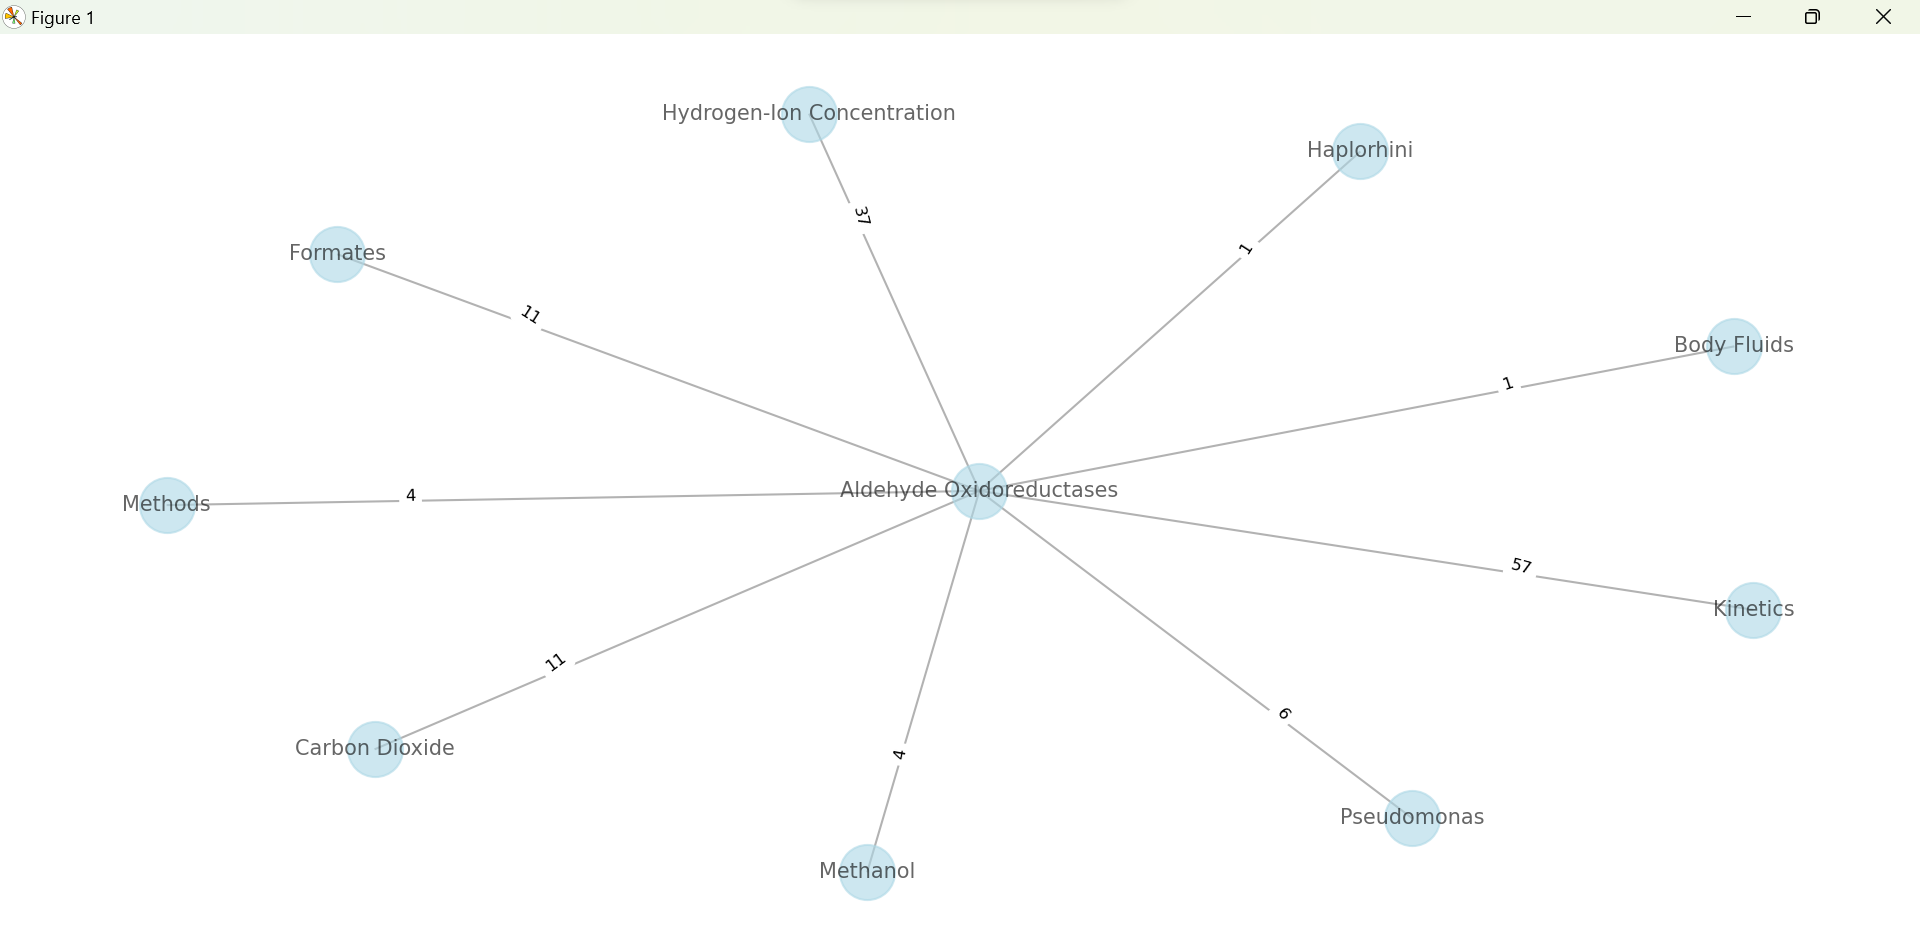
\includegraphics[width=\linewidth]{images/test_graph_creation.png}
    \caption{A small test graph to sanity check the graph creation process.}
    \label{fig:test_graph_creation}
\end{figure}

\subsection{Sub-Graph Creation} 

For all of the following systems I would create, I would want to be able to test them on smaller sub-graphs so that I could run them faster for testing purposes and to easily evaluate if they are functioning correctly. However, as can be seen in \Cref{fig:test_graph_creation}, the data when used for creating these graphs is organised by how the pairs of tags were initially formed. I was concerned that this data trend would continue into the graphs, resulting in strange and unhelpful graphs like \Cref{fig:test_graph_creation}. Therefore I ran a test of creating a sub-graph from the before 2008 graph containing ten nodes. This graph can be seen in \Cref{fig:test_subgraph}. As can be observed in this graph, it is much more meaningful and contains more information of the relationships between each of the nodes present than was the case in \Cref{fig:test_graph_creation}. \\

\subsection{Filtering Graphs}

For making and evaluating my link predictions, I required certain features to my data. Firstly, in my after 2008 graph, I only wanted to have edges present that were not present in the before 2008 graph. That is to say, if the link between concepts A and C had already been established before the time-split, there is no value in predicting it. Furthermore, I only wanted to predict about nodes, or MeSH tags, that I had already seen in the before 2008 graphs. Therefore, I combed through the post 2008 graph and removed any edges that existed in the before 2008 graph and any nodes that did not. This resulted in a filtered after 2008 graph with 362987 edges and 9653 nodes. \\

\begin{figure}[h]
    \centering
    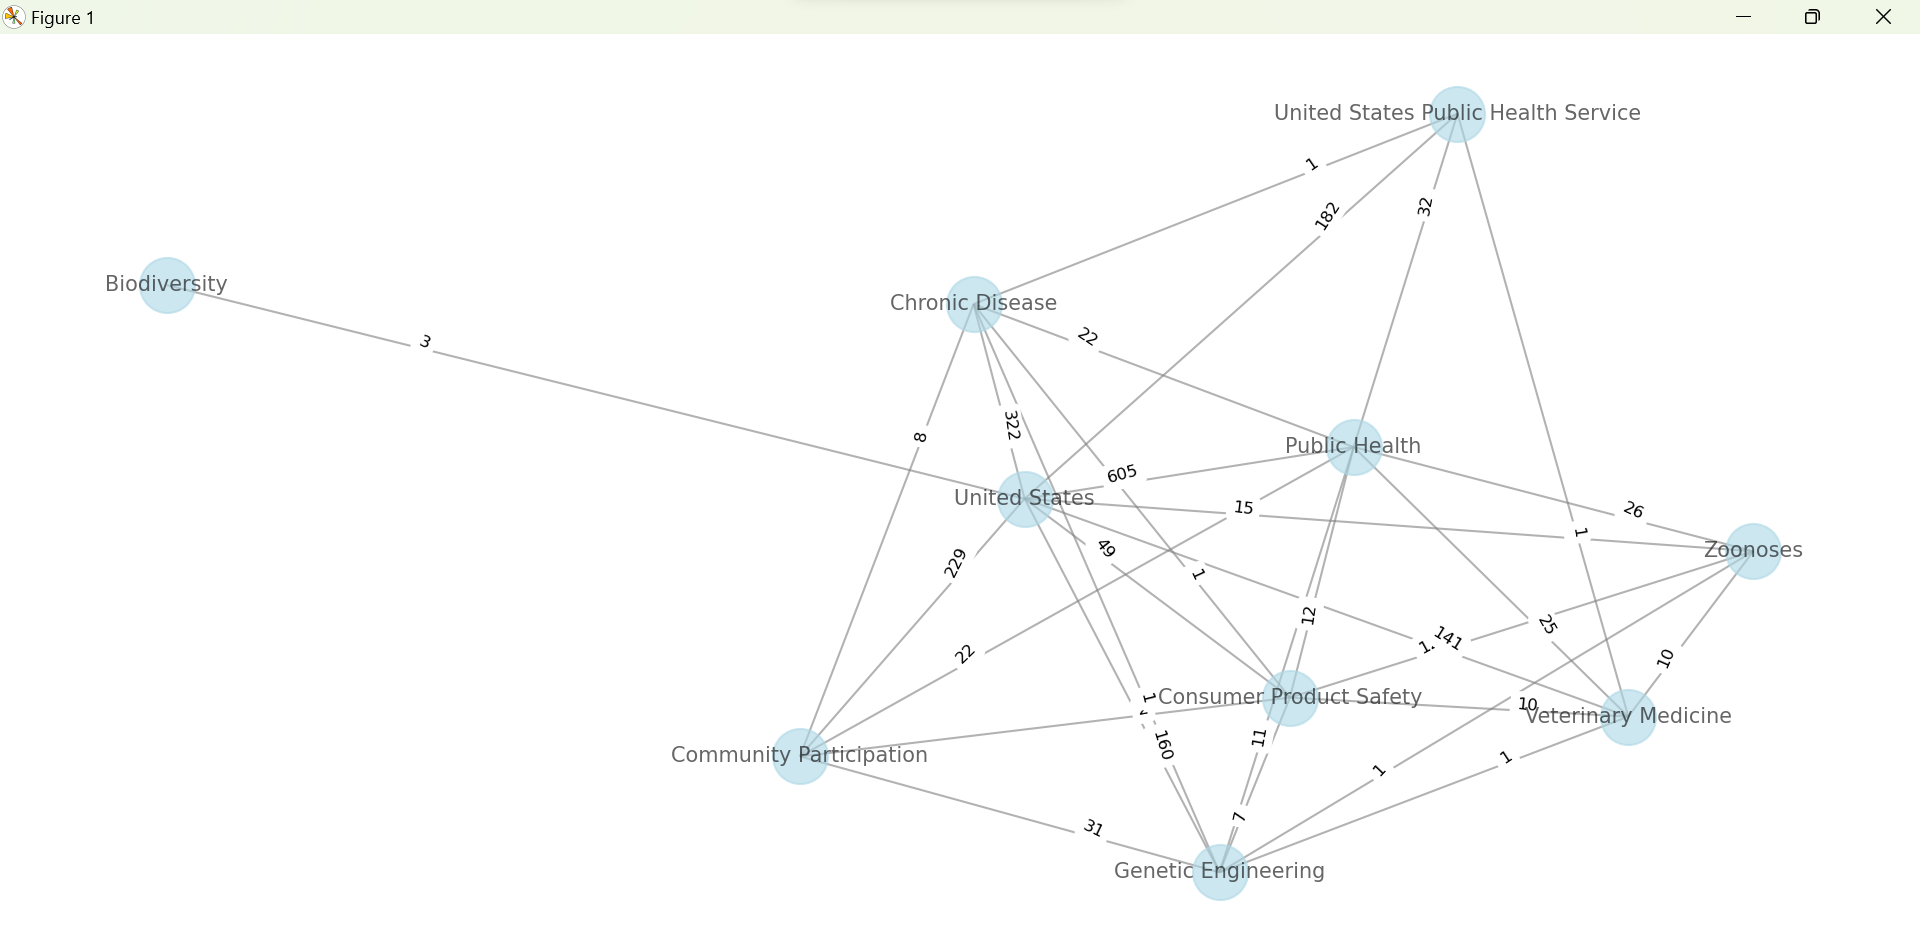
\includegraphics[width=\linewidth]{images/test_subgraph.png}
    \caption{A small test sub-graph to sanity check the sub-graphing process.}
    \label{fig:test_subgraph}
\end{figure}

\section{Swanson ABC}

\subsection{Initial Process}

The first prediction system I implemented was Swanson's ABC system. First, this required for each A node, getting a list of B nodes by returning the neighbours of that A node. At this stage we had the all of the concepts that co-occurred in articles with the MeSH tag represented by that A node. The next step was to get the neighbours of each of these B nodes, however there was an additional stipulation here. These new neighbours had to be filtered for any of the other B nodes. This is because, to qualify as a C node, the node in question must not already be connected to the A node. Once this filtering was done, a set of C nodes and B nodes was complete for each A node. \\

\subsection{Sorting C nodes}

On its own, the system so far simply returns all possible C nodes with no ability to evaluate how good each of these C nodes is as a prediction of a future link. To evaluate these predictions, they need to be sorted by some system which can rank them. With the data provided by our system there are three ways that these C nodes can be ranked. \\

The first approach is to use the total weight of the edges that connect each C node to the original A node. An easy mistake to make here is to only consider the edges from the C node and sum these. However, the weight of the edges between the A node and the B nodes should also be included here. For example, if A and C are connected by nodes B1 and B2, the total weight of the connection between A and C will be the summed weight of edges AB1, AB2, CB1 and CB2. This can formalised as follows, where $n$ is the number of B nodes the connect A and C.
\begin{center}
    $C_{\text{weight}} = \sum_i^n ((AB_i)_{\text{weight}} + (CB_i)_{\text{weight}})$ \\
\end{center}

The next sorting system will use the number of connecting B nodes between each A and C node. This means that each possible C MeSH tag will simply have a value attributed to it equal to the number of MeSH tags that appear in an article with both it and the original A tag. For example, if A and C are connected by nodes B1 and B2, the C node will be evaluated with a frequency score of 2. This can formalised as follows, where set $B$ is the set of nodes that connect A and C.
\begin{center}
    $C_{\text{frequency}} = |B| $\\
\end{center}

The final method of ranking these C nodes is to combine the previous two systems. To do this I multiplied the two values together. I opted not to sum them together as this would make the frequencies fairly irrelevant in the calculation. This calculation can be formalised as follows, given the previous two equations we have just defined. The only modification made, is that the square root of the value is taken so as to keep the numbers more readable.
\begin{center}
    $C_{\text{combined}} = \sqrt{|B|(\sum_i^n ((AB_i)_{\text{weight}} + (CB_i)_{\text{weight}}))}$\\
\end{center}

\subsection{Sanity check}

To ensure that these systems were producing the results I wanted I conducted a sanity check on them using the small, ten node graph seen previously in \Cref{fig:test_subgraph}. I used the node United States Public Health Service node as the A to evaluate on this graph. This node had five C nodes, giving a range of different frequencies, weights and combined scores. Here are the frequencies as an example of how the C nodes can be sorted. These scores can be compared to \Cref{fig:test_subgraph} to see that the system correctly evaluates them.\\

\begin{table}[h]
\centering
\caption{Data Sorted by Frequency}
\begin{tabular}{|c|c|c|}
\hline
\textbf{Position} & \textbf{Frequency} & \textbf{Name} \\ \hline
1 & 4 & Genetic Engineering \\ \hline
2 & 4 & Consumer Product Safety \\ \hline
3 & 3 & Community Participation \\ \hline
4 & 3 & Zoonoses \\ \hline
5 & 1 & Biodiversity \\ \hline
\end{tabular}
\end{table}

\subsection{Evaluation Implementation}

Hits@K was the evaluation method used to measure the prediction capabilities of these different sorting systems. Hits@k evaluates the accuracy of predicted links in Knowledge Graphs for missing link prediction by assessing the model's ranking of true versus false missing links. It gauges the percentage of correct predictions within the top k ranked links, with a higher Hits@k value signifying superior performance in missing link prediction. This assessment method is widely employed in link prediction tasks to gauge the efficacy of various models and algorithms. 

\section{Graph Neural Network}

\subsection{PyTorch}

PyTorch, created by Facebook AI Research and other labs, blends fast and flexible GPU-accelerated libraries with an easy Python interface. It's great for quickly trying out new ideas and works with many types of deep learning models. It allows for coding in python but with the efficiency usually reserved for other more demanding languages. PyTorch is well integrated with other packages such as SciPy, NumPy and NetworkX, enabling seamless combinations with them. Furthermore, PyTorch is widely used in data science reading enabling for better collaboration of research and replication of results. \\

Within PyTorch is a sub library called PyTorch Geometric. This library is designed to allow straightforward creation and training of GNNs for structured data such as graphs. It is this library that contains the aforementioned function that allows for the easy translation from NetworkX graphs to PyTorch Data structures. In addition, it contains a variety of functionality to allow for deep learning on graphs such as batch loaders, graph convolution networks (GCNs) and GNNs. \\

\subsection{Starting building}

Despite these benefits, I found it incredibly hard to get into PyTorch. Complicated tutorials, dense documentation and endless functions within functions made for a near insurmountable entry to the software. This lead to a lot of time being spent going round in circles without producing anything, just trying to fix bugs within bugs and creating more problems than I was solving. To rectify this spiral, I opted to copy a tutorial from Medium written by Jan Eric Lenssen and Matthias Fey, that builds a link prediction model on a heterogeneous graph. This tutorial follows a PyTorch tutorial on link prediction but adds to it explanations of functions and concepts to aid with development and understanding. \\

Translating this code to fit my data was very challenging. Their train\_loader using PyTorch Geometric LinkNeighbourLoader did not accept their data format, and when I tried to fit it to my data, once again did not work there either. Moving forwards with the development, I had to change their data set up to accommodate my graphs. The biggest hurdle in this process was translating it from heterogeneous to homogeneous. I had assumed that this would be a straight forward process given that I would be reducing the information down. However large components of the system were built on the assumption and utilisation of the different aspects of this data. This caused endless problems and seriously slowed down development. Weeks were spent pouring over documentation, changing a couple of lines, re-running code, no change, repeat, some change, new bug, repeat. A serious problem faced was the difficulty in bug fixing PyTorch code due to the black box nature of so many of the core functions. Eventually, a break through enabled the system to train successfully and produce predictions. \\

The next problem faced was the absence of negative sampling. In the provided tutiorial, this had been done by the batch loader and the link splitter, a function that divided the data into training and test sets, and so was not used in my system which was already split. This obviously resulted in extreme predictions being made due to the system not seeing any negative data. This was resolved by using PyTorch Geometric's negative sampling function and adding negative edges to both the training and the testing data sets. \\

\subsection{Performance Evaluation}

To evaluate the performance of this system I used the area under the curve (AUC) of the receiver operating characteristic curve (ROC). An ROC curve graphically represents a classification model's performance across different classification thresholds, plotting both the True Positive Rate (TPR) and the False Positive Rate (FPR). \\

The TPR is defined as: 

\begin{center}
    $\text{TPR} = \frac{\text{TP}}{\text{TP} + \text{FN}}$ \\
\end{center}

And the FPR is defined as: 

\begin{center}
    $\text{FPR} = \frac{\text{FP}}{\text{FP} + \text{TN}}$
\end{center}

The meaning of these variables is as follows. TP represents the true positives, FN represents the false negatives, FP represents false positives and TN represents true negatives. An ROC curve depicts the relationship between TPR and FPR across various classification thresholds. Decreasing the classification threshold results in more items being classified as positive, thereby elevating both False Positives and True Positives. \\ 

\begin{figure}[h]
    \centering
    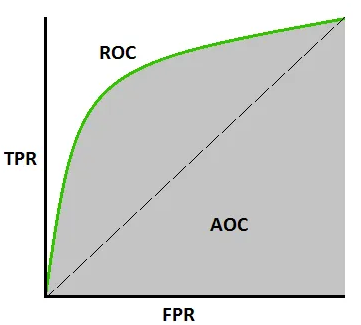
\includegraphics[width=0.5\linewidth]{images/roc_auc.png}
    \caption{image from: https://towardsdatascience.com/understanding-auc-roc-curve-68b2303cc9c5}
    \label{fig:roc_auc}
\end{figure}

To evaluate what the graph shown in \Cref{fig:roc_auc} tells us, we use the AUC, which tells us the chance that a true example would be evaluated by the model as higher than a false example. The AUC varies between 0 and 1, where an AUC of 0.0 signifies a model with predictions entirely incorrect, while an AUC of 1.0 denotes a model with predictions entirely correct. AUC is advantageous for two primary reasons: It assesses the ranking quality of predictions rather than their absolute values, and it also evaluates the model's prediction quality regardless of the chosen classification threshold. \\

\subsection{Performance Improvement}

The GNN system that I had built now faced a performance problem, it was not very good. Not only was it not very good, it was not better than randomly guessing. On multiple runs the AUC hovered around 0.5, which is to say it has a 50-50 chance of guessing correctly if a link exists or not. \\

To try to improve this performance I systematically walked through

\begin{itemize}
    \item pytorch
    \item using tutorial
    \item Converting to homogeneous
    \item Negative sampling
    \item bug fixing problems
    \item Trying to improve performance
    \item Sanity check
    \item Implementing evaluation
\end{itemize}

\section{Matrix Factorisation}
\begin{itemize}
    \item using tutorial
    \item Converting to homogeneous
\end{itemize}

\section{Compare Systems}
\begin{itemize}
    \item 
\end{itemize}

\section{Combine Systems}
\begin{itemize}
    \item 
\end{itemize}

\chapter{Evaluation} 

\chapter{Conclusion}    

\begin{appendices}

\chapter{Appendices}

Typical inclusions in the appendices are:

\begin{itemize}
\item
  Copies of ethics approvals (required if obtained)
\item
  Copies of questionnaires etc. used to gather data from subjects.
\item
  Extensive tables or figures that are too bulky to fit in the main body of
  the report, particularly ones that are repetitive and summarised in the body.

\item Outline of the source code (e.g. directory structure), or other architecture documentation like class diagrams.

\item User manuals, and any guides to starting/running the software.

\end{itemize}

\textbf{Don't include your source code in the appendices}. It will be
submitted separately.

\end{appendices}

%==================================================================================================================================
%   BIBLIOGRAPHY   

% The bibliography style is abbrvnat
% The bibliography always appears last, after the appendices.

\bibliographystyle{abbrvnat}

\bibliography{l4proj}

\end{document}
